% P3, Figure F0 (manuscript Fig. 1): how the results of the paper depend on one another (roadmap), in the style of the
% roadmap figure of the companion MSSP manuscript: plain shaded boxes on a fixed grid, each with a bold result, a one-line
% statement and the equation, result and section that give it; arrows point to dependent results; a dashed box for the
% evaluation and a list of the steps of use. Redrawn 18/10/2026.
% Width 164 mm (text width of the journal 165 mm). Every box has an inner sep of 2pt (0.7 mm per side), so a box spans
% its text width plus 1.4 mm: two columns of text width 78.6 mm (x = 0 to 80, 84 to 164), three boxes of 52 mm in the
% fourth row (x = 0 to 53.4, 55.3 to 108.7, 110.6 to 164), full-width boxes 162.6 mm. Equation, theorem and section
% numbers follow main.aux of 19/10/2026 (Sections 6-7 split into case study and results; 7.6 added 20/10/2026). Compile: xelatex F0_khung.tex -> F0_khung.pdf (copied to F0.pdf).
\documentclass{article}
\usepackage{newtxmath}
\usepackage[no-math]{fontspec}
\setmainfont{TeX Gyre Termes}
\usepackage{array}
\usepackage{tikz}
\usetikzlibrary{arrows.meta}
\pagestyle{empty}
\begin{document}
\setbox0=\hbox{\fontsize{7pt}{8.4pt}\selectfont
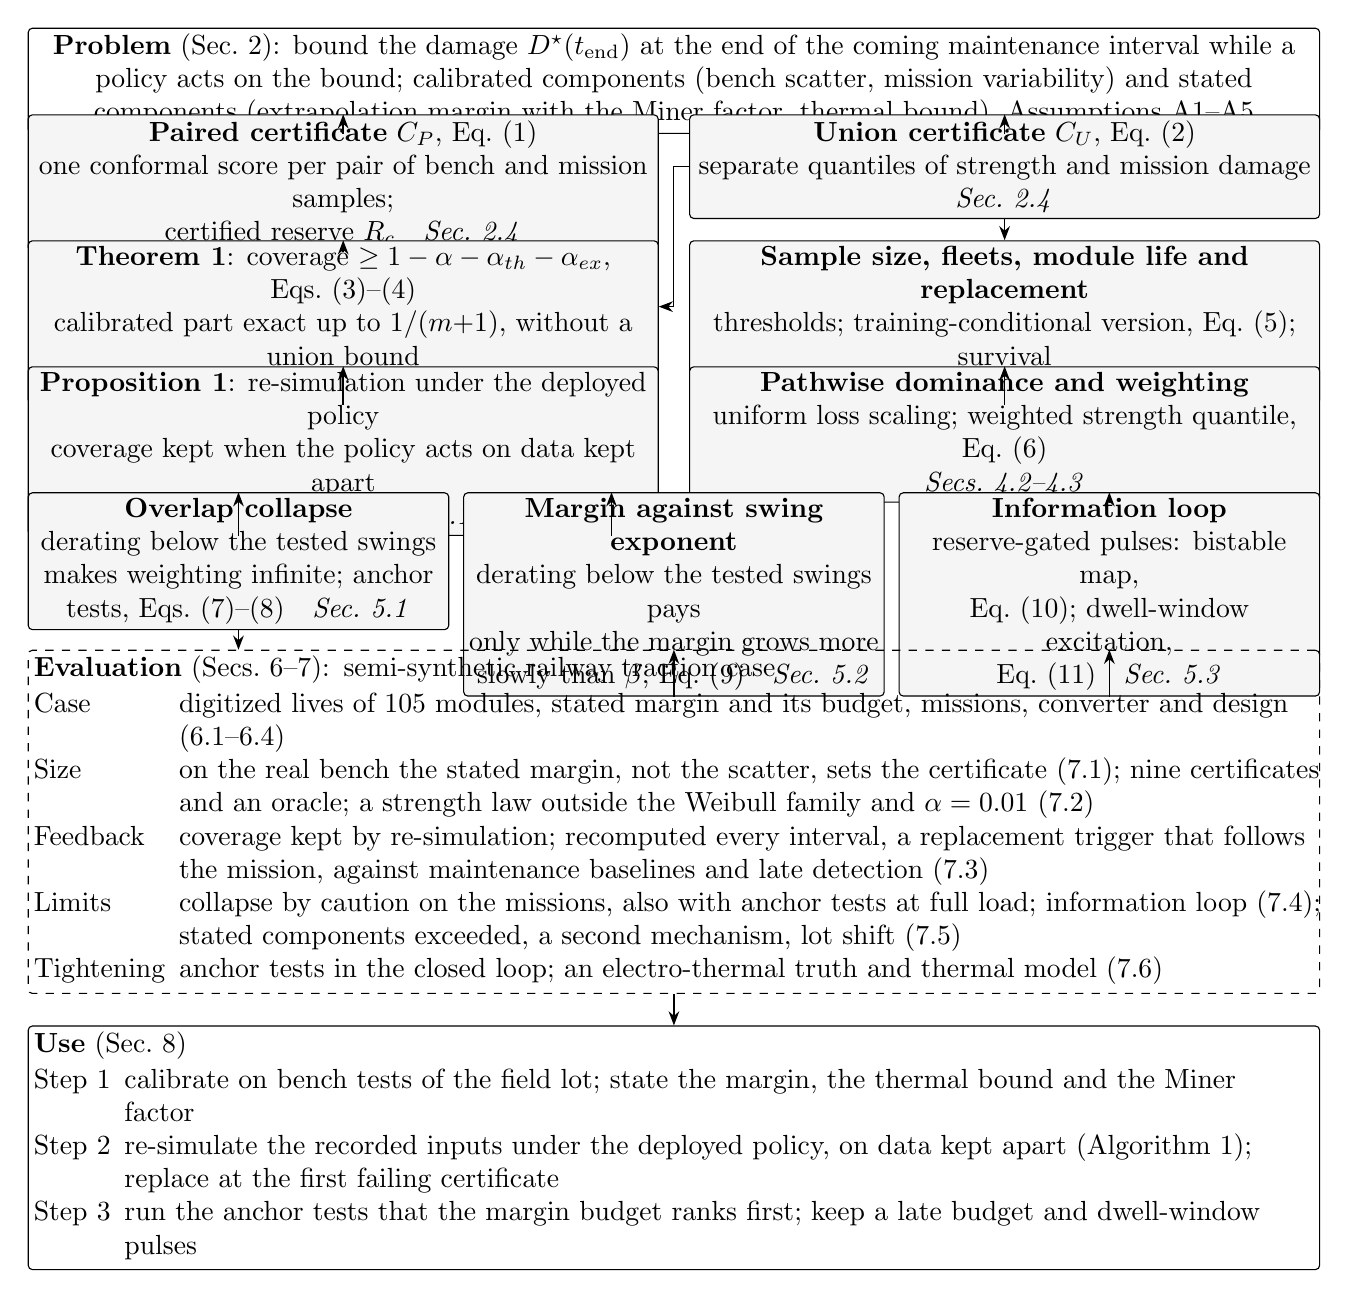
\begin{tikzpicture}[x=1mm, y=1mm,
    box/.style={draw, rounded corners=1.5pt, align=flush center, inner sep=2pt, anchor=north,
                execute at begin node={\hyphenpenalty=10000\exhyphenpenalty=10000},
                text width=#1, fill=black!4},
    box/.default=78.6mm,
    list/.style={draw, rounded corners=1.5pt, align=left, inner sep=2pt, anchor=north, text width=162.6mm},
    arr/.style={-{Stealth[length=1.8mm]}, semithick}]

% problem
\node[box=162.6mm, fill=white] (in) at (82,0)
  {\textbf{Problem} (Sec.~2): bound the damage $D^\star(t_{\mathrm{end}})$ at the end of the coming maintenance interval
   while a policy acts on the bound; calibrated components (bench scatter, mission variability) and stated components
   (extrapolation margin with the Miner factor, thermal bound), Assumptions~A1--A5};

% row 1
\node[box, minimum height=12mm] (pair) at (40,-11)
  {\textbf{Paired certificate} $C_P$, Eq.~(1)\\
   one conformal score per pair of bench and mission samples;\\
   certified reserve $R_c$\quad \textit{Sec.~2.4}};
\node[box, minimum height=12mm] (union) at (124,-11)
  {\textbf{Union certificate} $C_U$, Eq.~(2)\\
   separate quantiles of strength and mission damage\\
   \textit{Sec.~2.4}};

% row 2
\node[box, minimum height=12mm] (thm) at (40,-27)
  {\textbf{Theorem 1}: coverage $\ge1-\alpha-\alpha_{th}-\alpha_{ex}$, Eqs.~(3)--(4)\\
   calibrated part exact up to $1/(m{+}1)$, without a union bound\\
   \textit{Sec.~3.1}};
\node[box, minimum height=12mm] (size) at (124,-27)
  {\textbf{Sample size, fleets, module life and replacement}\\
   thresholds; training-conditional version, Eq.~(5); survival\\
   \textit{Secs.~3.2--3.3}};

% row 3
\node[box, minimum height=12mm] (prop) at (40,-43)
  {\textbf{Proposition 1}: re-simulation under the deployed policy\\
   coverage kept when the policy acts on data kept apart\\
   Algorithm~1; \textit{Sec.~4.1}};
\node[box, minimum height=12mm] (dom) at (124,-43)
  {\textbf{Pathwise dominance and weighting}\\
   uniform loss scaling; weighted strength quantile, Eq.~(6)\\
   \textit{Secs.~4.2--4.3}};

% row 4: collapse by caution
\node[box=52mm, minimum height=15.5mm] (ov) at (26.7,-59)
  {\textbf{Overlap collapse}\\
   derating below the tested swings\\
   makes weighting infinite; anchor\\
   tests, Eqs.~(7)--(8)\quad \textit{Sec.~5.1}};
\node[box=52mm, minimum height=15.5mm] (mg) at (82,-59)
  {\textbf{Margin against swing exponent}\\
   derating below the tested swings pays\\
   only while the margin grows more\\
   slowly than $\beta$, Eq.~(9)\quad \textit{Sec.~5.2}};
\node[box=52mm, minimum height=15.5mm] (il) at (137.3,-59)
  {\textbf{Information loop}\\
   reserve-gated pulses: bistable map,\\
   Eq.~(10); dwell-window excitation,\\
   Eq.~(11)\quad \textit{Sec.~5.3}};

% evaluation
\node[list, dashed] (ev) at (82,-79)
  {\textbf{Evaluation} (Secs.~6--7): semi-synthetic railway traction case\\[1pt]
   \begin{tabular}{@{}l@{\enspace}>{\raggedright\arraybackslash}p{146mm}@{}}
   Case & digitized lives of 105 modules, stated margin and its budget, missions, converter and design (6.1--6.4)\\
   Size & on the real bench the stated margin, not the scatter, sets the certificate (7.1); nine certificates and an
          oracle; a strength law outside the Weibull family and $\alpha=0.01$ (7.2)\\
   Feedback & coverage kept by re-simulation; recomputed every interval, a replacement trigger that follows the
              mission, against maintenance baselines and late detection (7.3)\\
   Limits & collapse by caution on the missions, also with anchor tests at full load; information loop (7.4); stated
            components exceeded, a second mechanism, lot shift (7.5)\\
   Tightening & anchor tests in the closed loop; an electro-thermal truth and thermal model (7.6)
   \end{tabular}};

% use
\path (ev.south) ++(0,-4) node[list] (use)
  {\textbf{Use} (Sec.~8)\\[1pt]
   \begin{tabular}{@{}l@{\enspace}>{\raggedright\arraybackslash}p{150mm}@{}}
   Step 1 & calibrate on bench tests of the field lot; state the margin, the thermal bound and the Miner factor\\
   Step 2 & re-simulate the recorded inputs under the deployed policy, on data kept apart (Algorithm~1); replace at the
            first failing certificate\\
   Step 3 & run the anchor tests that the margin budget ranks first; keep a late budget and dwell-window pulses
   \end{tabular}};

% derivation
\draw[arr] (in.south -| pair.north) -- (pair.north);
\draw[arr] (in.south -| union.north) -- (union.north);
\draw[arr] (pair) -- (thm);
\draw[arr] (union.west) -- ++(-2,0) |- ([yshift=2mm]thm.east);
\draw[arr] (union) -- (size);
\draw[arr] (thm) -- (prop);
\draw[arr] (size) -- (dom);
\draw[arr] (prop.south -| ov.north) -- (ov.north);
\draw[arr] ([xshift=-6mm]prop.south east) -- ([xshift=-6mm]prop.south east |- mg.north);
\draw[arr] (dom.south -| il.north) -- (il.north);
% into the evaluation and the use
\draw[arr] (ov.south) -- (ov.south |- ev.north);
\draw[arr] (mg.south) -- (mg.south |- ev.north);
\draw[arr] (il.south) -- (il.south |- ev.north);
\draw[arr] (ev.south) -- (use.north);
\end{tikzpicture}}
\pdfpagewidth=\dimexpr\wd0+4pt\relax
\pdfpageheight=\dimexpr\ht0+\dp0+4pt\relax
\shipout\vbox{\vskip-1in\vskip2pt\hbox{\hskip-1in\hskip2pt\box0}}
\end{document}
